\documentclass{sig-alternate}

\usepackage{url}
\usepackage{amsmath}
\usepackage{graphicx}
\usepackage{subfigure}
\usepackage{threeparttable}
\usepackage{pdflscape}
\usepackage{array}
\usepackage{color}

\begin{document}

\title{The Bug Catalog of the Maven Repository Ecosystem}

\numberofauthors{5} 

\author{
% 1st. author
\alignauthor
Dimitris Mitropoulos\\
       \affaddr{Athens University of Economics and Business}\\
       \affaddr{Department of Management Science and Technology}\\
       \email{dimitro@aueb.gr}
% 2nd. author
\alignauthor Vassilios Karakoidas\\
       \affaddr{Athens University of Economics and Business}\\
       \affaddr{Department of Management Science and Technology}\\
       \email{bkarak@aueb.gr}
% 3rd. author
\alignauthor Panos Louridas\\
       \affaddr{Athens University of Economics and Business}\\
       \affaddr{Department of Management Science and Technology}\\
       \email{louridas@aueb.gr}
\and  % use '\and' if you need 'another row' of author names
% 4th. author
\alignauthor Georgios Gousios\\
       \affaddr{Delft University of Technology}\\
       \affaddr{Software Engineering Research Group}\\
       \email{G.Gousios@tudelft.nl}
% 5th. author
\alignauthor Diomidis Spinellis\\
       \affaddr{Athens University of Economics and Business}\\
       \affaddr{Department of Management Science and Technology}\\
       \email{dds@aueb.gr}
}

\maketitle
\begin{abstract}
The abstract is coming
\end{abstract}

\category{D.2.4}{Software Engineering}{Software/Program Verification}[Statistical methods]
\category{D.2.5}{Software Engineering}{Testing and Debugging}[Code inspections and walk-throughs]
\category{D.2.7}{Software Engineering}{Distribution, Maintenance, and Enhancement}[Version control]

\terms{Static Analysis, Software Ecosystems}

\keywords{Maven Repository, FindBugs, Software Bugs}

\section{Introduction}
\label{sec:intro}

In this paper we present a dataset produced after
analyzing a large software ecosystem to detect
software bugs. For our research we used
{\it FindBugs},\footnote{\url{http://findbugs.sourceforge.net/}}
a static analysis tool that examines bytecode to detect software bugs and has already been used in
research~\cite{AP10,SHP06}.
Specifically, we ran FindBugs on all the project
versions of all the projects that exist in the
{\it Maven Central Repository}\footnote{\url{http://mvnrepository.com/}}
(approximately 265{\sc gb} of data.

\section{Data Collection Experiment}
\label{sec:exp}
Body.

\section{Repository Statistics}
\label{sec:repo}
Repo stats.

\begin{figure}[t]
	\centering
	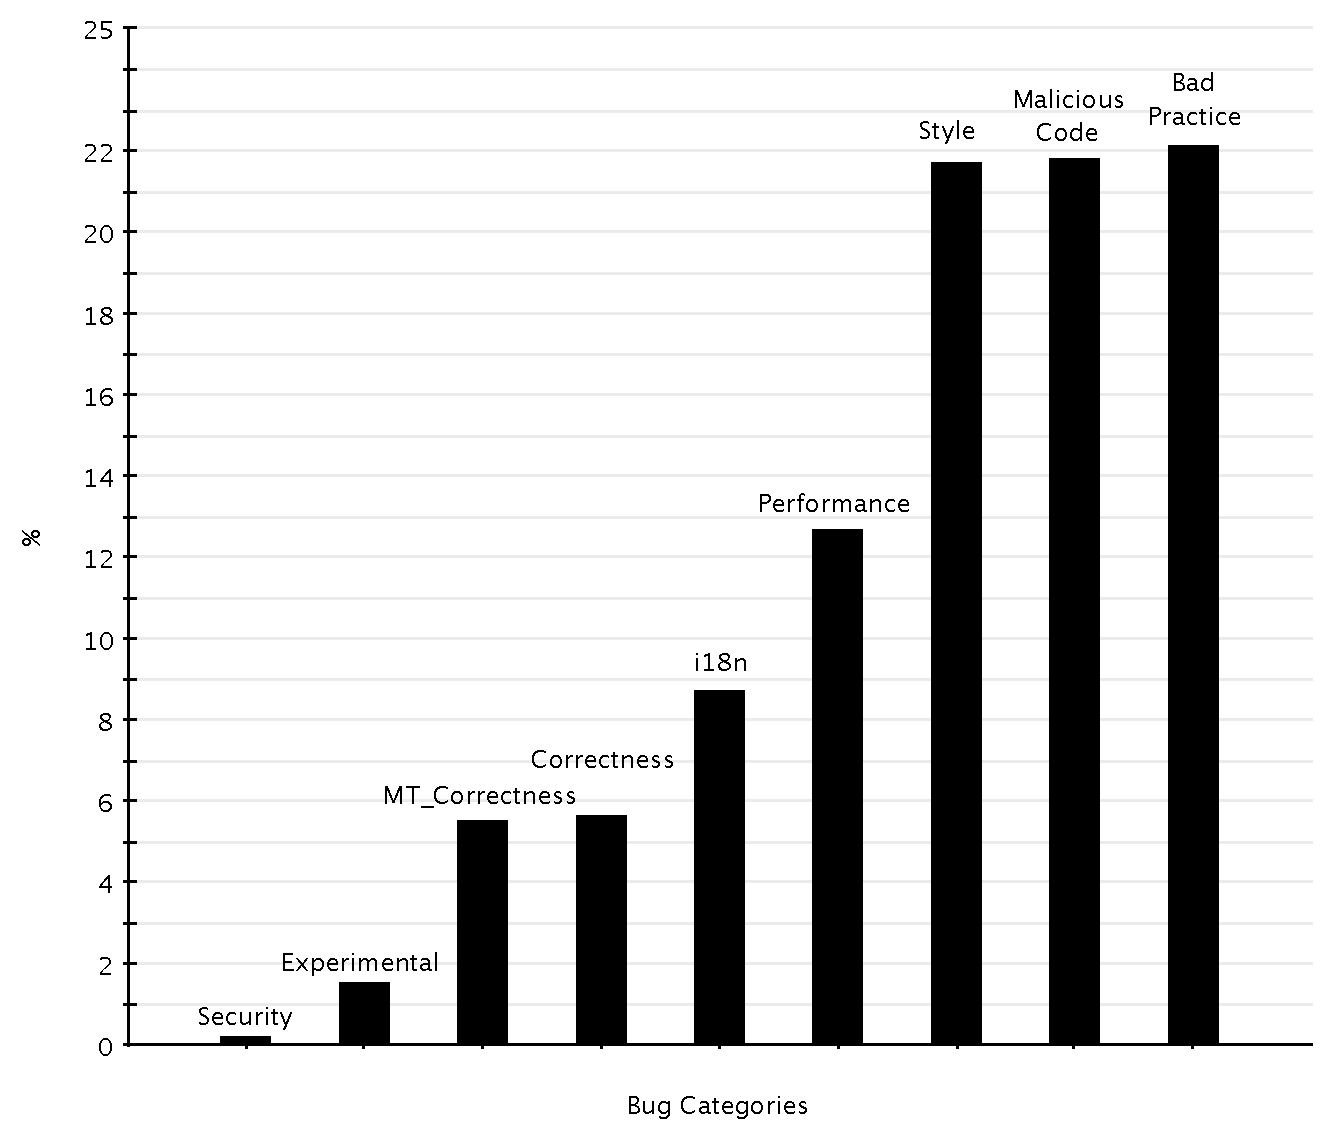
\includegraphics[scale=0.38]{figures/bug_percent}
	\caption{Bug percentage in Maven repository.}
	\label{fig:bug-per} 
\end{figure}

\section{Initial Findings}
\label{sec:find}
Findings.

\section{Tools}
\label{sec:exp}
Tools.

\section{Related Work}
\label{sec:rel}

\section{Conclusions}
\label{sec:conc}

\section{Acknowledgments}
possible acks.

\bibliographystyle{abbrv}
\bibliography{msr}  
\end{document}
